\section{Hardware}

This section is dedicated to show all the chosen electronic components and how they work together. As described earlier the PCB containing all the components will be manufactured by Seeedstudio. They manufacture PCBs with other hardware components and they sell quite a number of different breakout boards and other developpement parts. A request made by CHIC managing team was to source as many components as possible at Seeedstudio. Of course not all components needed were available by them so some of the components are from different sources.

The project was basically building a tablet. However time constraints did not allow the devellopment of a tablet from scratch. There for it was decided to build an add-on to an existing processing unit.

There are a number of different devellopment/tinkering boards available. The most famous one might be the raspberry Pi, although quite capable it seemed a little limited for this application (clocked at 700 mhz for the raspberry pi 1). Another problem was that the raspberry pi is not completely open source. Indeed its schematics and gerber files are not available. One of the requirements of the CHIC project was that it was necessary to work with a totally open source/open hardware platform. For these reasons the raspberry pi was discarded.

 Another famous board was chosen: the beagle bone black. Which will further be refered to as the BBB. This board clocked at 1 GHz seemed quite capable. There was lots of documentation, a wide community, and especially it is completelly open source hardware and software.

In fig.\ref{fig:hardware dependencies} the different components of the device are described.

\begin{figure}[!htb]
    \centering
    \includegraphics[width=0.7\textwidth,keepaspectratio]{chap/hardFig/overall_hardware_dependecies}
    \caption{Hardware components dependencies.}
    \label{fig:hardware dependencies}
\end{figure}

%///////////////////////// BBB //////////////////////////////////

\clearpage

\subsection{Beaglebone Black}
The BBB uses an ARM processor from Texas Instruments, the AM335X. It is clocked at 1GHz.

\begin{figure}[!htb]
    \centering
    \includegraphics[width=0.7\textwidth,keepaspectratio]{chap/hardFig/bbb.png}
    \caption{Beaglebone black.}
    \label{fig:bbb}
\end{figure}
The BBB capabilities include:
\begin{itemize}
  \item{ AM335x 1GHz ARM® Cortex-A8 }
  \item{512MB DDR3 RAM}
  \item{4GB 8-bit eMMC on-board flash storage}
  \item{Ethernet}
  \item{2x 46 pin headers}
  \item{Open source}
  \item{On board Power Management IC}
  \item{micro Sd card reader}
  \item{Ethernet}
  \item{micro HDMI output}
\end{itemize}
The main interface of the BBB are the 92 pins. Many pins can be configured in different modes. The pins and connection are listed in fig.\ref{fig:pin modes}.
\clearpage


%\begin{figure}[!htb]
\begin{sidewaysfigure}[h]
    \centering
    \includegraphics[width=0.9\textwidth,keepaspectratio]{chap/hardFig/BBB_pins_sch}
    \caption{Pin usage of the BBB.}
    \label{fig:pin modes}
%\end{figure}
\end{sidewaysfigure}

\clearpage

%///////////////////////// SCREEN //////////////////////////////////


\subsection{Screen and Touchscreen}
At the current state of the prototype the main function is to view images and text. Therefore a good screen with realistic colors is necessary to have a good user experience.
First a resistive touchscreen BBB cape (4DCAPE-70T by 4D systems) available from Seeedstudio was ordered to see how its was made and to see if the resistive technology was applicable to the project. Quickly the resistive touchscreen reveiled to be unsuitable to manipulate photos. Especially the very well known “swipe” gesture to move from one photo to another was impossible to do with the resistive touchscreen.
This screens colors were coded on 16 bits and the viewing angle was quite bad. It was decided to use a capacitive touchscreen and more colors if possible. A screen found on Mouser was chosen. It had good documentation and especially there was an existing driver for the touchscreen IC in the linux kernel planned to run on the BBB.
 The screen is actually a package containing the screen and its driver, the touch-screen and its driver and the backlight LED array. This package can be seen in fig.\ref{fig:screen package}

 \begin{figure}[!htb]
     \centering
     \includegraphics[width=0.5\textwidth,keepaspectratio]{chap/hardFig/newhaven_screen_image}
     \caption{Screen package.}
     \label{fig:screen package}
 \end{figure}

 Individual components are discribed in the following sub chapters.

\subsubsection{Screen}
The screen is the NHD-7.0-800480EF-ATXV\#-CTP from Newhaven Display. The specifications of the screens are listed bellow.
\begin{itemize}
  \item {7" Diagonal}
  \item{Resolution: 800xRGBx480}
  \item{24 bit digital RGB interface}
  \item{White led backlight}
  \item{55-65$^{\circ}$ Top-bottom viewing angle }
  \item{70 $^{\circ}$ left-rigth viewing angle}
\end{itemize}
The viewing angle is better than with the 4d cape and the colors more realistic.

\subsubsection{Touchscreen}

\begin{itemize}
  \item {Capacitive touch panel with built-in Focaltech ft5x06 controller}
  \item {i2c interface}
  \item {multi-touch compatible (up to 5 simultanious touches)}
  \item {linux kernel 3.14 compatible}
\end{itemize}
The touchpanel is very smooth and reactive. The swipe gesture works very well.

\subsubsection{Backlight}
\label{chap: backlight}
The backlight is a quite bright white led array consisting of 5x3 LEDs. the configuration can be seen in fig.\ref{fig:backlight_led}

\begin{figure}[!htb]
    \centering
    \includegraphics[width=0.5\textwidth,keepaspectratio]{chap/hardFig/backlight_led_circuit}
    \caption{Backlight LED array configuration.}
    \label{fig:backlight_led}
\end{figure}

This LED array requires 60 mA at 16 V to operate. This power is taken directly from the 3.3v of the BBB and boosted to the required voltage by FAN5333A LED driver from Fairchild semiconductors.
This IC is a general purpose LED driver which can be controller with a PWM imput.
The implementation of the FAN5333B is pictured in fig.\ref{fig:backlight driver schematics}.

\begin{figure}[!htb]
    \centering
    \includegraphics[width=0.7\textwidth,keepaspectratio]{chap/hardFig/backlight_led_driver_sch}
    \caption{FAN5333B Backlight LED driver implementation.}
    \label{fig:backlight driver schematics}
\end{figure}

From the data sheet the resistance R30 regulates the current. The net EHRPWMMOA is connected to a pwm pin on the BBB. The brightness of the screen will be adjustable from the website interface.

%///////////////////////// WIRELESS //////////////////////////////////

\subsection{Wireless Communication}
\label{chap:wireless com}
The device has to connect to the internet over a WLAN to download new messages from the website. The WL1835 chip from Texas instruments was chosen. This IC integrates WlAN, 4.1 bluetooth and BLE. An important point is that TI provides support for the linux kernel planned to run on the AM335x ARM® Cortex-A8.

The chip is provided in a 100-pin MOC package. The pin designation is seen in fig.\ref{fig:wl1835 pin designation}.

\begin{figure}[!htb]
    \centering
    \includegraphics[width=0.5\textwidth,keepaspectratio]{chap/hardFig/100_pin_MOC_wl1835_package}
    \caption{Wl1835 pin designation.}
    \label{fig:wl1835 pin designation}
\end{figure}

To operate the wl1835 needs a few external components. Among others an oscillator and antennas are necessary to for proper operation.
The integration of this chip was inspired by a layout example provided by TI as well as by the layout of an existing BBB cape which can be found here \url{http://boardzoo.com/index.php/beaglebone/beaglebone-wl1835mod-w-chip-antenna.html}.

The implementation is displayed in fig.\ref{fig:wl1835 chip}



\begin{figure}[!htb]
    \centering
    \includegraphics[width=1\textwidth,keepaspectratio]{chap/hardFig/wl1835_chip_sch}
    \caption{Wl1835 implementation.}
    \label{fig:wl1835 chip}
\end{figure}

\subsubsection{Wlan}
The chip supports the IEEE standards 802.11a/b/g/n. This means it can provide up to 100 MPs with UDP and up to 80 MPs with TCP.
It uses a 4 bit SDIO interface to communicate with the BBB. The BBB has 2 SDIO interfaces which are used to communicate with the micro sd card and the onboard EMMC. Therefore using the wl1835 means that access to the emmc is no longer possible. This is not a big issue as the operating system can be located on the sd card.


\subsubsection{Bluetooth}
The Wl1835 provides 4.1 bluetooth and low energy bluetooth capabilities. Uart host controlled interface is used to communicate through this interface.

The bluetooth interface is not used currently. It is integrated thinking of future development (see chap.\ref{chap: next steps}).

\subsubsection{Power management}
The WL1835 is quite power hungry, it can pull up to about 500 mA (more in calibration mode) of current and requires both 3.3V and 1.8V sources to operate. Therefore it has its own linear regulators which pull their current directly from the battery. For the 1.8V the TPS73618DBVR low voltage dropout regulator is used. It can output a maximum of 400 mA at 1.8V. For the 3.3V the TL1963ADCQT LDO is used. The maximum output current is this time 1.5 A which should be well over the maximum current consumption of the chip.


\begin{figure}[!ht]
    \centering
    \includegraphics[width=0.7\textwidth,keepaspectratio]{chap/hardFig/wl1835_power_sch}
    \caption{Wl1835 power management implementation.}
    \label{fig:power management}
\end{figure}

\subsubsection{Buffering}
As the signals that come in and out of the wl1835 are 1.8V and the BBB only works with 3.3V, a bidirectional Voltage-Level translator was needed. The same ones which were implemented in the existing wl1835 cape(see chapter \ref{chap:wireless com}) were chosen. The TXS0108EPWR from TI.

The implemention of these voltage converters is displayed in fig.\ref{fig:buffering chip}.

\begin{figure}[!ht]
    \centering
    \includegraphics[width=0.7\textwidth,keepaspectratio]{chap/hardFig/wl_1835_buffer_sch}
    \caption{TXS0108EPWR buffering chip implementation.}
    \label{fig:buffering chip}
\end{figure}

\subsubsection{Antennas}
This chip can handle two antennas although only one is compulsory. Again following the TI design guide as well as the schematics of the wl1835 BBB cape mentioned in chapter \ref{chap:wireless com} we implemented a dual antenna design. A ceramic chip was used for the on board antennas. The layout and custom footprints designed for this part are further described in chap.\ref{chap:pcb}.

%///////////////////////// FRONT LED //////////////////////////////////

\subsection{Front LED}

The LED is there to inform the user of a new message. As it is only a notification LED and a 20 mA warm white LED is enough. Another PWM pin of the BBB is used to make the LED blink.

%///////////////////////// ACCELEROMETER //////////////////////////////////

\subsection{Accelerometer}

A ADXL345 accelerometer from Analog Devices and distributed by Seeedstudio was used. It is mainly used to detect in which current orientation the device is. The screen is then turned accordingly. It may be used for further applications (see chap.\ref{chap: next steps}).

The accelerometer measures on three axis, has very low power consumption (as low as 23 \textmu A in measurement mode) and can be interfaced by i2c or spi. The former is used.

Implementation is portrayed in figure\ref{fig:acc}.
\begin{figure}[!ht]
    \centering
    \includegraphics[width=0.7\textwidth,keepaspectratio]{chap/hardFig/acc_sch}
    \caption{Accelerometer implementation.}
    \label{fig:acc}
\end{figure}
%//////////////////////// BATTERIES AND CHARGER //////////////////////////////////

\subsection{Batteries and charger}
The battery is a 3.7V Lithium-ion battery with a capacity of 6000mAh from Seeedstudio. The voltage of such batteries range from 3.7V to 4.2V which is in the range of input voltage of the BBB.
Seeedstudio also sell a li-ion battery charger and wireless power transmission coils. The battery charger is based on the CN3065 chip. It is a complete constant-current/constant voltage linear charger for single cell Li-ion and Li Polymer rechargeable batteries.

The power transmission coils are ready to use out of the box. They provide a constant 5V output of up to 600 mA.
The receiver coil is directly connected to the charging chip via an smd JST 2 pin connector soledered to the PCB. The transmitter coil is powered by a micro USB port.

\begin{figure}[!ht]
    \centering
    \includegraphics[width=0.7\textwidth,keepaspectratio]{chap/hardFig/wireless_charger}
    \caption{Wireless power transmission coils.}
    \label{fig:wireless charger}
\end{figure}

%///////////////////////// POWER MANAGEMENT //////////////////////////////////

\subsection{Power management}

The power source of the device is of course the battery. From the battery the power is channeled into two main groups. The BBB and the wl1835 wireless chip. The BBB provides power to the different components via its on board PMIC while the wireless chip has its dedicated PMIC. This is due to the great amount of current the wl1835 potentialy needs. It also requires a 1.8V source which the BBB doesn't provide. The power flow is detailed in figure \ref{fig:power flow}.

\begin{figure}[!ht]
    \centering
    \includegraphics[width=0.7\textwidth,keepaspectratio]{chap/hardFig/vesta_power_management}
    \caption{Eelctrical flow from the wall outlet to the different components of the device.}
    \label{fig:power flow}
\end{figure}



%///////////////////////// PCB //////////////////////////////////

\subsection{PCB}
\label{chap:pcb}
The PCB was designed in Altium Designer 15. Unfortunatly at this stage no prototype of the PCB has been made. All the components apart the wl1835 have been tested with the BBB on a breadboard. The complex package of the wl1835 chip prevents from connecting it to the BBB with wires. The cape mentionned in chap.\ref{chap:wireless com}as source for the wl1835 implementation.

\subsubsection{Overall description}

As can be seen in figures \ref{fig:4ds cape} and \ref{fig:vesta cape} both boards are quite similar. Indeed both boards have components on only one side to be able to stick the board on the back of the screen metal casing. The board is fixed to the case by 4 screws inserted in the mounting holes on the PCB.
Male smd headers on which the BBB is inserted are soldered to the PCB. The friction between the 92 pins and the headers is enough to hold the BBB in place.

\begin{figure}[h]
    \centering
    \includegraphics[width=0.7\textwidth,keepaspectratio]{chap/hardFig/4d_cape}
    \caption{Existing BBB cape with 7" inch screen and resistive touchscreen.}
    \label{fig:4ds cape}
\end{figure}

\begin{figure}[!ht]
    \centering
    \includegraphics[width=0.7\textwidth,keepaspectratio]{chap/hardFig/rendu_pcb_trois_quarts}
    \caption{Rendering of the pcb of the Vesta device.}
    \label{fig:vesta cape}
\end{figure}


The PCB is composed of four layers. The layer thicknesses, copper thicknesses as well as materials and all other rules were mainly dictated by Seeedstudios fabrication guidelines. The layers are described in table.\ref{tab:layer description}.

\begin{table}[!htbp]
  \begin{center}
    \begin{tabular}{|l|r|r|r|}%p{5cm}|}
      \hline
        Layer name & type & Material & Thickness [mm] \\ \hline \hline
        Top Overlay & Overlay & & \\ \hline
        Top solder & solder mask & surface material & 0.01 \\ \hline
        Component side & signal & copper & 0.03 \\ \hline
        Dielectric 1 & Dielectric & FR-4 & 0.2 \\ \hline
        Ground & GND & copper & 0.018\\ \hline
        Dielectric 1 & Dielectric & FR-4 & 1.1 \\ \hline
        Power & VCC & copper & 0.18 \\ \hline
        Dielectric 1 & Dielectric & FR-4 & 0.2 \\ \hline
        Bottom side & signal & copper & 0.035 \\ \hline
        Bottom solder & solder mask & surface material & 0.01 \\ \hline
        Bottom overlay & & &  \\ \hline

    \end{tabular}
  \end{center}
  \caption {Pcb layer description} \label{tab:layer description}
\end{table}

The power plane is set to the 3.3v of the BBB as it is the most used power line. The wl1835 3.3V and 1.8V power lines are located on the component side layer.

\begin{figure}[h]
    \centering
    \includegraphics[width=0.7\textwidth,keepaspectratio]{chap/hardFig/pcb_all_layers}
    \caption{Pcb layer stack and component placement.}
    \label{fig:pcb layer stack}
\end{figure}

The red traces in figure \ref{fig:pcb layer stak} are on the top component layer. Most of the traces are located on this layer. The blue traces are located on the bottom component layer. The blue traces are mainly the LCD 24 bit interface.

In figure \ref{fig:pcb pour} a polygon pour has been added as well as via stitching.

\begin{figure}[h]
    \centering
    \includegraphics[width=0.7\textwidth,keepaspectratio]{chap/hardFig/pcb_polygon_pour}
    \caption{Pcb polygon pour and via stitching.}
    \label{fig:pcb pour}
\end{figure}

\subsubsection{Antennas}
The chip antennas are the ANT016008LCD2442MA1 from TDK. The datasheet and previously mentioned examples were used to design the custom footprint.
The main considerations described by the aforementioned sources for the antennas to have maximum efficiency are:

\begin{itemize}
  \item {the antennas are orthogonal to each other}
  \item {They must be distanta of >76 mm which is a half wave length}
  \item {RF traces must have 50-\textOmega impedance}
  \item {RF traces must not have sharp corners}
  \item {RF traces must have via stitching on the ground plane beside the RF trace on both sides}
  \item {RF traces must be as short as possible. The antenna, RF traces, and module must be on the edge of the PCB product in consideration of the product enclosure material and proximity}
\end{itemize}

\begin{figure}[!htb]
    \centering
    \includegraphics[width=0.5\textwidth,keepaspectratio]{chap/hardFig/antenna_footprint}
    \caption{PCB antenna custom footprint.}
    \label{fig:wl1835 pcb antennas}
\end{figure}

Following the guidelines of the manufacturer the antennas were placed on the edge of the pcb, via shielding was applied and they were set more than the minimum distance appart. They also slightly stick out of the pcb so that they are not over the metal casing of the screen. This implementation is shown in figure \ref{fig:pcb antennas implement}.

\begin{figure}[!htb]
    \centering
    \includegraphics[width=0.5\textwidth,keepaspectratio]{chap/hardFig/antenna_implementation}
    \caption{PCB antenna implementation.}
    \label{fig:pcb antennas implement}
\end{figure}

\clearpage
\subsection{Assembly}
In Figure~\ref{fig:assembly} an assembly of the components of the device is shown.
\begin{sidewaysfigure}[!htb]
    \centering
    \includegraphics[width=0.9\textwidth,keepaspectratio]{chap/designFig/AssemblageVestaB_290415}
    \caption{Device assembly.}
    \label{fig:assembly}
\end{sidewaysfigure}

\subsection{Cost estimates}
\begin{table}[!htbp]
  \begin{center}
    \begin{tabular}{|l|r|r|}%p{5cm}|}
      \hline
        Component & number of units & Price per unit [CHF] \\ \hline \hline
        Screen & 1 & 90 \\ \hline
        BBB & 1 &  45 \\ \hline
        wl1835 & 1 &  25 \\ \hline
        Battery & 1 & 20 \\ \hline
        PCB & 1 & 20 \\ \hline
        Case parts & 1 & 10 \\ \hline
        Wireless coils & 1 & 20  \\ \hline
        Resistors & 40 & 4 \\ \hline
        capacitors & 20 & 4 \\ \hline
        Inductors & 5 & 2 \\ \hline
        miscallenous ICs & 10 & 15 \\ \hline
        Connectors & 10 & 10 \\ \hline
        micro SD card & 1 & 10 \\ \hline
        usb charger & 1 & 10 \\ \hline \hline
        Total & 94 & 285\\ \hline

    \end{tabular}
  \end{center}
  \caption {Prototype cost estimates} \label{tab:cost estimates}
\end{table}

The costs in table \ref{tab:cost estimates} are the prices paid for single components. The screen takes up nearly one third of the cost but can easily be lowered.
